\documentclass{standalone}
\usepackage{tikz}
\usetikzlibrary {arrows.meta}
\pagestyle{empty}

\begin{document}
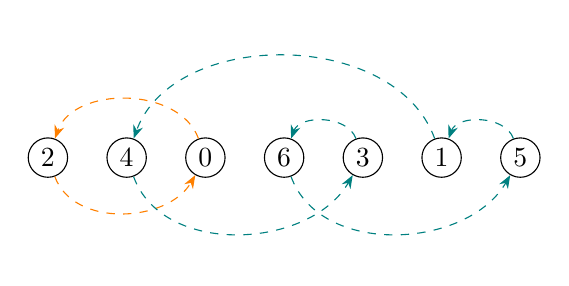
\begin{tikzpicture}

\tikzstyle{every node}=[draw,shape=circle,minimum size=0.5cm,inner sep=0pt,anchor=center];

% Draw the splay tree nodes
\node (n0) at (2,0) {0};
\node (n1) at (5,0) {1};
\node (n2) at (0,0) {2};
\node (n3) at (4,0) {3};
\node (n4) at (1,0) {4};
\node (n5) at (6,0) {5};
\node (n6) at (3,0) {6};


\tikzset{every edge/.append style = {-Stealth,dashed,gray}};

% Visitation: normal edition
\path[every node/.style={font=\sffamily\small}]
  (n2) edge[out=290,in=240,orange] (n0)
  (n0) edge[out=110,in=70,orange] (n2)
  (n4) edge[out=290,in=240,teal] (n3)
  (n3) edge[out=110,in=70,teal] (n6)
  (n6) edge[out=290,in=240,teal] (n5)
  (n5) edge[out=110,in=70,teal] (n1)
  (n1) edge[out=110,in=70,teal] (n4);


\end{tikzpicture}
\end{document}
